\documentclass[12pt]{jhwhw}
\author{Ian Malerich}
\title{Math 331: Homework 0}
\usepackage{amsmath, amsfonts, amsthm, amssymb, scrextend, setspace, framed, tikz}
\usetikzlibrary{arrows, positioning}
\onehalfspacing

\begin{document}
\raggedright{}

%% Problem 1
\problem{}

	Reproduce the text and figure exactly as it appears, including the rectangular border.

\solution
\begin{spacing}{1.0}

%% My default frame had a lot more padding than yours
%% I assume this isn't what you used
%% but it does look quite a bit closer
\FrameSep4pt
\begin{framed}

	This is an inline equation: $x+y=3$. \\
	This is a displayed equation:
	$$
		x + \frac{y}{z - \sqrt{3}} = 2.
	$$
	This is how you can define a piece-wise linear function: \\
	$$ 
		f(x) = 
		\begin{cases}
			3x + 2 & \text{if } x<0 \\
			7x + 2 & \text{if } x\ge 0 \text{ and }x<10 \\
			5x + 22 & \text{otherwise.}
		\end{cases} 
	$$
	This is a matrix: \\
	%% Your "matrix" (table) had cells taller than wide
	%% not really sure why, mine don't do that by default
	%% I found this array stretch replicates it nicely
	%% so I'm a dirty cheater, so sue me
	\renewcommand{\arraystretch}{1.4}
	$$
		\begin{tabular}{|c|c|c|c|}
			\hline
			9 & 9 & 9 & 9 \\
			\hline
			6 & 6 & 6 & \\
			\hline
			3 &   & 3 & 3 \\
			\hline
		\end{tabular}
	$$
	This is a figure incorporated in a LaTeX file \\
	$$
	%% Marvel in how beautiful my perfect circle graph is
	%% it's perfect in ever way
	%% I want extra credit
	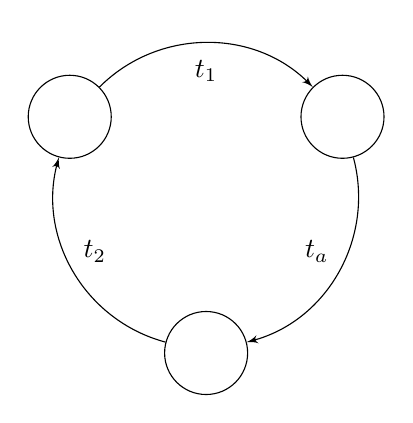
\begin{tikzpicture}
		\tikzset{vertex/.style = {shape=circle, draw, minimum size=3.0em}}
		\tikzset{edge/.style = {->,> = latex'}}

		\node[vertex] (a) at (-1.73205, 1.0) {};
		\node[vertex] (b) at (1.73205, 1.0) {};
		\node[vertex] (c) at (0,-2) {};

		\draw[edge] (a) to[bend left=45] node[midway, below = 1mm] {$t_1$} (b);
		\draw[edge] (b) to[bend left=45] node[midway, above left] {$t_a$} (c);
		\draw[edge] (c) to[bend left=45] node[midway, above right] {$t_2$} (a);

	\end{tikzpicture}
	$$

\end{framed}
\end{spacing}

%% Problem 2
\problem{}

	Show that $\mathbb{N}$ and $\mathbb{Z}$ are equinumerous.

\solution
\begin{proof}
	
	The sets $\mathbb{N}$ and $\mathbb{Z}$ are equinumerous iff 
	$|\mathbb{N}| = |\mathbb{Z}|$. By definition of cardinality,
	this is true iff there exists some function $f$ which forms a bijection between
	the given sets.
	\bigbreak
	Consider the function $f: \mathbb{N} \rightarrow \mathbb{Z}$ defined as follows
	$$
		f(x) = 
		\begin{cases}
			0 & \text{if }x = 1 \\
			x/2 & \text{if $x$ is even} \\
			-(x-1)/2 & \text{otherwise}
		\end{cases}
	$$
	\bigbreak
	\textbf{Injective.} \\
	Assume $f(x) = f(y)$
	\bigbreak

	case $f(x) = f(y) = 0$:
	\begin{addmargin}{2em}
		Note that x is clearly not even, as $f(x) = x/2 > 0$. \\
		Further, x is not odd and greater than 1 as $(x-1) > 0 \Rightarrow f(x) = -(x-1)/2 < 0$. \\
		Therefore, we conclude $x = 1$ as $f(1) = 0$.
		By the same logic, $y = 1$. \\
		Thus we have that $x = y = 1$.
	\end{addmargin}

	case $f(x) = f(y) > 0$:
	\begin{addmargin}{2em}
		Note that neither $x, y$ cannot be 1, else $f(x) = f(y) = 0$. Further $x, y$ must be even, else $f(x) < 0$. \\
		Thus, $f(x) = f(y)$ \\
		$\Rightarrow x/2 = y/2$ \\
		$\Rightarrow 2x/2 = 2y/2$ \\
		$\Rightarrow x = y$.
	\end{addmargin}

	case $f(x) = f(y) < 0$:
	\begin{addmargin}{2em}
		Following the same argument as above, we note that $x,y$ must both be odd and $\neq 1$. \\
		Thus, $f(x) = f(y)$ \\
		$\Rightarrow -(x-1)/2 = -(y-1)/2$ \\
		$\Rightarrow -(-2)(x-1)/2 = -(-2)(y-1)/2$ \\
		$\Rightarrow x-1 = y-1$ \\
		$\Rightarrow x-1+1 = y-1+1$ \\
		$\Rightarrow x = y$ \\
	\end{addmargin}

	\bigbreak
	\textbf{Surjective.} \\
	let $y \in \mathbb{Z}$
	\bigbreak

	case $y = 0$:
	\begin{addmargin}{2em}
		choose $x\in \mathbb{N} = 1$, then $f(x) = f(1) = 0$.
	\end{addmargin}

	case $y > 0$:
	\begin{addmargin}{2em}
		choose $x = 2y$, where $y > 0 \wedge y \in \mathbb{Z} \Rightarrow y \in \mathbb{N} 
		\Rightarrow x = 2y \in \mathbb{N}$. \\
		Further note that $x = 2y$ is even. \\
		Thus $f(x) = f(2y) = 2y/2 = y$. \\
	\end{addmargin}

	case $y < 0$:
	\begin{addmargin}{2em}
		choose $x = -2y+1$, where $y < 0 \wedge y \in \mathbb{Z} \Rightarrow -y \in \mathbb{N}
		\Rightarrow x = -2y+1 \in \mathbb{N}$ \\
		Further note that $x = -2y+1$ is odd. \\
		Thus $f(x) = f(-2y+1) = -(-2y+1-1)/2 = -(-2y)/2 = 2y/2 = y$.
	\end{addmargin}

	\bigbreak
	Thus, as $f$ forms a bijection on $\mathbb{N}$ and $\mathbb{Z}$ we conclude that 
	$\mathbb{N}$ and $\mathbb{Z}$ are equinumerous.
\end{proof}

%% Problem 3
\problem{}

	Let $f: S \rightarrow S$ be a total function. Prove that if $S$ is infinite, 
	$f$ can be (a) one-one without being onto, and (b) onto without being one-one.

\solution

\begin{proof}
For both examples, assume $f: \mathbb{N} \rightarrow \mathbb{N}$, where $\mathbb{N}$ serves as an 
example of an infinite set $S$.

\part

	Define $$f(x) = x+1$$ \\
	Note that $f$ is defined $\forall x\in \mathbb{N}$ thus $f$ is total. \\
	If we let $f(x) = f(y)$ then $x+1 = y+1 \Rightarrow x=y$. Clearly $f$ is one-one. \\
	However, consider $f(x) = 1$, then $x+1 = 1 \Rightarrow x=0$ but $0\not\in \mathbb{N}$. \\
	Therefore $f$ is not onto as $1\in \mathbb{N}$ is not reachable from its (infinite) domain.

\part

	Define 
	$$
	f(x) = \begin{cases}
		1 & x \text{ is even} \\
		x/2 & x \text{ is odd} \\
	\end{cases}
	$$
	Note that $f$ is defined $\forall x\in \mathbb{N}$ thus $f$ is total. \\
	Let $y\in \mathbb{N}$, then $f(2y) = (2y)/2 = y$, noting 2y even, therefore $f$ is onto. \\
	However, $f(1) = f(3) = f(5) = \dotsb = 1$, clearly $f$ is not one-one.
\end{proof}

%% Problem 4
\problem{}

	Show that the relation $R$ defined 

	$$
		\forall m,n \in \mathbb{N}, (m,n)\in R \iff (m-n) \text{ mod } 3 = 0
	$$

	is an equivalence relation, and describe its equivalence classes.

\solution
\begin{proof} An equivalence relation is one that is reflexive, symmetric, and transitive\dots \\

\bigbreak
\textbf{Reflexive.} \\
	let $a\in \mathbb{N}$ \\
	$(a - a) \text{ mod }3 = 0 \text{ mod } 3 = 0 \Rightarrow (a, a) \in R$

\bigbreak
\textbf{Symmetric.} \\
	let $a,b\in \mathbb{N}$ \\
	assume $(a,b)\in R$ then $(a-b) \text{ mod } 3 = 0$ \\
	note that $(a-b) = -(b-a)$ \\
	then $(b-a) \text{ mod } 3 = -(a-b) \text{ mod } 3 = -((a-b) \text{ mod } 3) = -0 = 0$ \\
	therefore $(b,a) \in R$.

\bigbreak
\textbf{Transitive.} \\
	let $a,b,c\in \mathbb{N}$ \\
	assume $(a,b)\in R\ \wedge\ (b,c)\in R$. \\
	then $(a-b) \text{ mod } 3 = 0\ \wedge\ (b-c) \text{ mod } 3 = 0$. \\
	consider $(a-c) \text{ mod } 3 = (a-c+b-b) \text{ mod } 3 = ((a-b)+(b-c)) \text{ mod } 3$ \\
	we can distribute the modulus operator\dots \\
	$(a-c)\text{ mod }3 = ((a-b)\text{ mod }3)+((b-c)\text{ mod }3)\text{ mod }3$ \\
	$= (0 + 0)\text{ mod }3 = 0\text{ mod }3 = 0$ \\
	therefore $(a,c)\in R$.

\end{proof}

Each equivalence class contains any numbers who's differences form multiples of 3.
Thus there are 3 equivalence class. Natural numbers who are offset by $3k$ from 0, those who are offset by $3k$
from 1, and those who are offset by $3k$ from 2 (for some $k \in \mathbb{N}$). \\
$\{0, 3, 6, 9, 12\dots\}$ \\
$\{1, 4, 7, 10, 13\dots\}$ \\
$\{2, 5, 8, 11, 14\dots\}$ \\

%% Problem 5
\problem{}

	Show that $\sum_{i=1}^{n} i^{2} = (2n+1)(n+1)n/6$.

\solution
\begin{proof} \textit{via induction on n}

\bigbreak
\textbf{Induction Basis.} \\
	let $n=1$ \\
	then $\sum_{i=1}^{n}i^{2} = n^2 = 1^2 = 1$ \\
	and $(2n+1)(n+1)n/6 = (2\cdot 1+1)(1+1)\cdot 1/6$ \\
	$= 3(2)/6 = 6/6 = 1$

\bigbreak
\textbf{Induction Basis.} \\
	$\exists\ k\in \mathbb{N} : \sum_{i=1}^{k} i^{2} = (2k+1)(k+1)k/6$. \\

\bigbreak
\textbf{Induction Step.} \\
\begin{spacing}{1.4}
	assume $\exists\ n\in \mathbb{N} : \sum_{i=1}^{n} i^{2} = (2n+1)(n+1)n/6$ via Induction Hypothesis.\\
	then $\sum_{i=1}^{n}i^{2} + (n+1)^2 = (2n+1)(n+1)n/6 + (n+1)^2$ \\
	$ = \sum_{i=1}^{(n+1)}i^{2} = (2n+1)(n+1)n/6 + n(n+2)+1$ \\
	$ = (2n+1)(n+1)n/6 + 6(n(n+2)+1)/6$ \\
	$ = ((2n^3 + 3n^2 + n) + (6n^2 + 12n + 6))/6$ \\
	$ = (2n^3 + 9n^2 + 13n + 6)/6$ \\
	$ = (2n+3)(n+2)(n+1)/6$ \\
	$ = \sum_{i=1}^{n+1}i^{2} = (2(n+1)+1)((n+1)+1)(n+1)/6$ \\

\end{spacing}
\end{proof}

\end{document}
